\documentclass[english]{article}

\usepackage[nodayofweek]{datetime}

%\title{\textbf{Title} \\subtitle}
%\author{Zhao Lyu}
%\date{2018-01-15}%change \today


\usepackage{amsmath, mathtools, amsfonts,amssymb,flexisym,enumitem,grffile,graphicx,tikz,subcaption,titling}
\usepackage{tikz}
\usepackage{tkz-euclide}
\usetkzobj{all}
\usepackage{wrapfig,blindtext,babel,calc}
%\usetikzlibrary{intersections,calc}
\usepackage{setspace}
\setlist[enumerate]{itemsep=0mm}
\graphicspath{{/home/user/Project199/Figures}}

\usepackage{amsthm}
\newtheorem*{definition*}{Definition}
\newtheorem{definition}{Definition}
\newtheorem{theorem}{Theorem}
\newtheorem*{theorem*}{Theorem}
\newtheorem*{lemma*}{Lemma}
\newtheorem{lemma}{Lemma}
\newtheorem*{claim*}{Claim}
\newtheorem{claim}{Claim}

\newcommand{\vol}{\operatorname{vol}}
\newcommand{\diam}{\operatorname{diam}}


\begin{document}

  \doublespacing %use setspace package
  %\maketitle{Refinement Strategy in 2 Dimension}
  \title{\textbf{Simplicial Mesh Refinement in Computational Geometry}}
  \author{Zhao Lyu}
  \maketitle
  \singlespacing

  \newpage %separate title and contents
  \pagenumbering{gobble}
  \tableofcontents
  \newpage
  \pagenumbering{arabic}

  \section{Introduction}
  One question in computational geometry is how to represent complicated geometric shapes as a composition of more simple shapes. For example, an area can be expressed as composition of triangles, and a volume can be written as a composition of tetrahedra. In this thesis, we discuss an important topic about such decompositions, namely the refinement of simplicial meshes.

One motivation for this topic is the numerical analysis of partial differential equations. While numerical methods simulate the behavior of a partial differential equation over some area, it is necessary  to represent the area on a computer first. This process is called triangulation, decomposing the area into simplices. Importantly, we sometimes may want to increase the resolution of this triangulation \cite{grosso1998hierarchical}. To do so, algorithms which perform simplicial mesh refinement are crucial and worthy of attention. Besides its application in particial differential equations, mesh refinement can also be applied in other fields, such as solving interpolation problems \cite{moore1992simplical}.

There are two main challenges in designing such algorithms. One is to maintain the stability of these simplices. In other words, unlimited to how many times a refinement is repeated, shapes of triangles should be bounded. That is, there should not exist any degenerating triangles, which refers to those with extremely small angles. One main reason why degenerating triangles should be avoided is that these triangles lead to ill-conditioned matrices in numerical methods for partial differential equations [CITATION NEED]. Another challenge is to  preserve the consistency of the triangulation. This means that two triangles either do not touch or only touch at a common edge or vertex, and the importance of this attribute is that an algorithm is expected to refine triangles consistently and successfully. In short, these two constrains make the development of algorithms for simplicial mesh refinement a challenging problem, because not all  ...

In this thesis, we discuss two applicable algorithms for mesh refinement in two dimensions. The first algorithm is called uniform refinement, classified as a global refinement \cite{bank1983some,bey2000simplicial,Bey1995}. Though its easy application and obvious qualification for stability and consistency bring a popularity to this refinement strategy, it fails to process some flexibility in refining simlicial meshes. This is because uniform refinement forces to refine the entire mesh at once. However, many applications demand the flexibility to refine the mesh only locally. Thus, another algorithm, called the newest vertex bisection, is introduced to obtain such flexibility for local mesh refinement. However, newest vertex bisection is not perfect either. While newest vertex bisection of a single triangle preserves stability, preservation of consistency becomes complicated. In detail, the problem is that bisecting one triangle may depend on bisection of another. This leads to a chain reaction, which can be understood as a recursion using a stack and traversing back only when a base case is touched. Therefore, the difficulty is to determine how many triangles are part of this chain reaction, and under which conditions this chain reaction ends. In other words, we need to find out when the algorithm terminates and how long it lasts. 

In conclusion, this thesis will introduce uniform refinement and newest vertex bisection in two dimensions for computational geometry, and prove their stability and consistency in application, and further discuss their potential limits and possible solutions.
...
  %\newpage

  \section{Basic Definition}
    We first recall definitions of linear transformation and translation, and further introduce affine transformations, which we will use to prove stability of uniform mesh refinement and bisection in sections later. Then we introduce basic notions which we will use to present mesh refinement and show how they would work out.

       \subsection{Translation, Linear Transformation and Affine Transformation}
      
      We define several classes of transformations that we frequently use.
      
      \begin{definition*}
        %$\textbf{Translation}$\\
         Let $\textbf{v}$ be a fixed vector. A $\textbf{translation}$ ${T}_v$ on a figure applies as ${T}_v (\textbf{p}) = \textbf{p} + \textbf{v}$, for any vector $\textbf{p}$ in the figure which we translate.
      \end{definition*}
      A $\textit{translation}$ moves every point of a figure or space by the same distance in the same direction. A translation ${T}$ can be represented by an addition of a constant vector to every point.


      \begin{definition*}
      %\paragraph{Linear transformation}
      Let ${V}$ and ${W}$ be vector spaces over the same field $\textbf{K}$. We say a function $\mathit{f}: {V} \rightarrow {W}$ is a $\textbf{linear transformation}$ if the following is satisfied:
      \begin{align*}
      \mathit{f}(\textbf{u} + \textbf{v}) &= \mathit{f}(\textbf{u}) + \mathit{f}(\textbf{v}) \qquad \forall \textbf{u}, \textbf{v} \in{V},\\
      \mathit{f}(c\textbf{u}) &= c\mathit{f}(\textbf{u}), \qquad \forall \textbf{u} \in{V}, ~c\in\textbf{K}.
      \end{align*}
      \end{definition*}
      In other words, a linear transformation is a mapping between two vector spaces which preserves the operations of vector addition and scalar multiplication. Moreover, if ${V}$ and ${W}$ are finite dimensional, we can represent the linear transformation ${f}$ by a matrix ${M}$. For example, if ${M}$ is an ${m} \times {n}$ matrix, then ${f}$ is a linear transformation from $\mathbf{R}^n$ to $\mathbf{R}^m$. 


      \begin{definition*}
      %\paragraph{Affine Transformation}
      An $\textbf{affine transformation}$ from $\mathbb{R}^n$ to $\mathbb{R}^n$ is of the form\\
      \begin{equation*}
      {F}(x) = {Ax} + {v}, \qquad {x}\in\mathbb{R}^n,
      \end{equation*}
      where ${A}\in\mathbb{R}^{n\times n}$ is a matrix, and  ${v}\in\mathbb{R}^n$ is a vector.\\
      \end{definition*}
      The inverse mapping of an affine transformation $F(x) = Ax + v$, is only defined if $A^{-1}$ exists, and we define the inverse mapping $F^{-1} = {x} \mapsto {A}^{-1}({x} - {v})$ is also an affine transformation.\\
      Affine transformation preserves points, lines and planes, but need not preserve point zero in a linear space in contrast to linear transformation. So we see that translations and linear transformations are affine, but the opposite is not true. Affine transformation helps carry results from one simplex to another simplex in our discussion, and more details are covered after introducing ${Simplices}$ and ${Triangulations}$ in the next section.



        \subsection{Simplices}
    In this section, we will introduce simplices and talk about its geometrical properties, such as diameter and volume. These information and notation are mainly from \cite{ciarlet2002finite}\cite{bey2000simplicial}
    \noindent
    \begin{definition*}
    A $k$-simplex $T \subseteq\mathbb{R}^n$ is a convex hull of $k+1$ vertices ${x}_0, \cdots, {x}_k \in \mathbb{R}^n$, which are affinely independent. We write 
    \begin{equation*}
    \begin{split}
    {T} & = [{x}_0, \cdots, {x}_k ]\\
    & := \left\{{x} = \sum\limits_{i=0}^k \lambda_i {x}_i \Bigm| \sum\limits_{i=0}^k \lambda_i = 1 \text{and} 0 \leqslant \lambda_i \leqslant 1, 0 \leqslant i \leqslant k \right\}\\
    & := \left\{\lambda_0{x}_0 + \cdots + \lambda_k{x}_k \Bigm| \sum\limits_{i=0}^k \lambda_i = 1 \text{and} 0 \leqslant \lambda_i \leqslant 1, 0 \leqslant i \leqslant k \right\}.
    \end{split}
    \end{equation*}
    \end{definition*}
    If $k = n$, we do not address the dimension of a $k$-simplex. 2-simplices are also called \emph{triangles}, and 3-simplices are called \emph{tetrahedra}.

    \begin{definition*}
    %\paragraph{Subsimplices}
    An  $l$-simplex ${S} = [{y}_0, \cdots, {y}_l]$ is called an \emph{$l$-subsimplex} of a $k$-simplex ${T} = [{x}_0, \cdots, {x}_k]$, if there exist indices $0 \leqslant {i}_0 \leqslant \cdots\leqslant{i}_l \leqslant k$ with ${y}_{i_{j}} = {x}_i$, for all $0 \leqslant j \leqslant l$.
    \end{definition*}
    Since there are $k+1$ vertices in a $k$-simplex $T$, and $l+1$ vertices in $l$-subsimplices $S$, the number of $l$-subsimplices of $k$-simplices is $\binom{k+1}{l+1}$.


    %\paragraph{Simplices Equality}
    Consider simplices $T = [{x}_0, \cdots, {x}_k]$ and $T' = [{y}_0, \cdots, {y}_k]$. We say these two simplices $T$ and $T'$ are equal, i.e. $T = T'$, if ${x}_i = {y}_i$ for $0 \leqslant i \leqslant k$. Note that the vertex ordering of simplex is fixed, so if two simplices $T$ and $T'$ denote the same set but with different vertex ordering, they are not equal; instead, we say that ${T}$ coincides with $T'$, i.e. $T \cong T'$.

    \paragraph{Simplices under Affine Transformation}\mbox{}\\
    Let $F$ be an affine transformation. 
    Instead of taking a single variable $x\in\mathbb{R}^n$ for affine transformation, we can take a subset S $\subseteq\mathbb{R}^n$, which contains $x\in\mathbb{R}^n$. Then the transformed set $S'$ is
    \begin{equation*}
    S\textprime= \left\{{F}(x) ~|~ x\in S \right\}.
    \end{equation*}
    Similarly, if we regard a k-dimensional simplex ${T} = [{x_0, \cdots, x_k}]$ as a subset of $\mathbb{R}^n$ then the image of ${T}$ under affine transformation is defined as
    \begin{equation*}
    \begin{split}
    {F}({T}) = \big[{F}(x_0), \cdots , {F}(x_k)\big]
    \end{split}
    \end{equation*}
    We can see that $F(T)$ is still a k-dimensional simplex. Let us write $T' = F(T)$. We might be curious about the relationship between simplices $T$ and $T'$. 
    %Since vertices of a simplex are in a specific given order, so different vertex ordering leads to different simplices. Therefore, there exists a unique affine transformation such that $T = T'$. 
    An important property of simplices is congruence.

    \begin{definition*}
    Two simplices $T$, $T'$ are defined to be congruent if they can be obtained from each other by rotation, mirroring, scaling, and translation, i.e. if there exists a scaling factor c $\in\mathbb{R}^{+}$, a translation vector $v\in\mathbb{R}^n$, and an orthogonal matrix $Q\in\mathbb{R}^{n\times n}$ such that
    \begin{equation*}
    T' = v + cQT
    \end{equation*}
    \end{definition*}
    \noindent
    %When the two simplices $T$ and $T'$ have same vertices but with different vertex ordering, we can translate it as $T' = F(T)$. Based on how we define the affine transformation, it is not hard to see that ${T} \cong {T}\textprime$. 
    Then we say that ${T}$ and ${T}\textprime$ are in a same congruence class. Formally, a cingruent class is an equivalent class of simplices under the congruence relation.
    \subsection{Shape Regularity Measure}%\mbox{}\\
    $\textit{Shape measure}$ offers an objective mathematical measure on the overall quality of a simplex, and this is helpful to explore the simplex regularity and to improve the quality of shapes of the elements. Different definitions are used for shape measure to present the quality of simplex, and we simply introduce the $\textit{geometric shape measure} ~\mu({T})$ of simplex ${T}$,  the one we use in this paper.

    \paragraph{Simplex Diameter and Volume}\mbox{}\\
    Let $T \in\mathbb{R}^n$ be a $k$-simplex where $k \leqslant n$, with vertices ${x}_0, \cdots, {x}_k \in\mathbb{R}^n$. We let $\diam(T)$ denote the diameter of $T$, and we see
    \begin{equation*}
    %\operator???
    \operatorname{diam}(T) = \max_{0\leqslant i\leqslant j\leqslant k} \| x_i - x_j \|
    \end{equation*}
    In other words, $\diam(T)$ is the longest distance between two vertices of $T$, which is the length of the longest edge of $T$. If $T$ is a single vertex, then $\diam(T) = 0$.\\

    \noindent
    Let $\vol^k$(${T}$) denote the k-dimensional volume of ${T}$. We have
    \begin{equation*}
    \operatorname{vol^k} (T) = \frac{1}{k!}\cdot|\det(x_1-x_0, x_2-x_0,\cdots, x_k-x_0)|
    \end{equation*}
    \noindent
    If k = 0, then $T$ is a 0-dimensional simplex, i.e., a vertex. By convention we have $\vol^0 ({T})$ = 1, which means that the volume of a single vertex is one.

    
    \paragraph{Shape Measure}\mbox{}\\
    Simplex diameter and volume are important to introduce shape measures. Here we define the {geometric shape measure} $\mu(T)$ of a $k$-simplex $T$ by
    \begin{equation*}
    \mu(T) = \frac{\operatorname{diam}(T)^k}{\operatorname{vol^k}(T)}, \quad\operatorname{vol^k(T) \neq 0}
    \end{equation*}
    If $\vol^k(T)$ = 0, then we define $\mu(T) = \infty$.\\
    
    To understand this definition, we can interpret $\mu(T)$ as a measurement of how different the two variables $\diam(T)^k$ and $\vol^k(T)$ are. For example, for a 2-dimensional simplex, i.e. a triangle, shape measure helps measure how narrow the triangle is. In other words, it measures how small the smallest angle of the triangle is. A triangle with a fixed diameter whose smallest angle gets smaller and smaller will look more and more like a one-dimensional line, and its shape measure will diverge to infinity.

    %\paragraph{Stability of a Simplex}\mbox{}\\
    

    %???
    \begin{figure}
    \centering
    \captionsetup{justification=centering}
    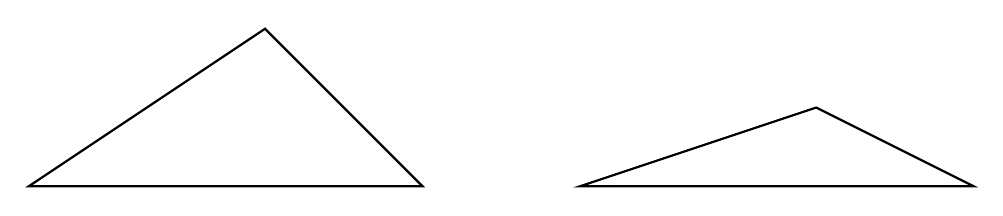
\begin{tikzpicture}
    \draw[thick] (0,0) -- (3,2) -- (5,0)-- cycle;
    \draw[thick] (7,0) -- (10,1) -- (12,0)-- cycle;
    %\path (1,1) coordinate (A) (2.5, 2.5) coordinate (B) (3, 1) coordinate (C)
    %\draw (A) -- (B) -- (C) -- cycle
    \end{tikzpicture}
    \caption{Good triangle(left) with smaller shape measure vs. \\Bad triangle(right) with larger shape measure}
    \label{Fig1}
    \end{figure}

    \begin{lemma}
    If $T$ and $T'$ are congruent simplices, then $\mu(T) = \mu(T')$.
    \label{lma0}
    \end{lemma}
    \begin{proof}
    Since $T$ is congruent to $T'$, by definition, we have $T' = v + cQT$, where $c\in\mathbb{R}^{+}$ is scaling factor, $v\in\mathbb{R}^n$ is a translation vector and $Q\in O(n)$ is an orthogonal matrix. In fact, we will show that scalings, translations, orthogonal transformation do not influence the shape measure of a simplex. 
    
    To be specific, when scaling a simplex $T$ by a non zero factor $c\in\mathbb{R}^{+}$ to obtain $T'$, we have 
    \begin{align*}
     \vol^k(T') &= \frac{1}{k!}\cdot|\det(cx_1-cx_0, cx_2-cx_0,\cdots, cx_k-cx_0)| \\
               &= \frac{c^k}{k!}\cdot|\det(x_1-x_0, x_2-x_0,\cdots, x_k-x_0)| = c^k\cdot \vol^k(T).
    \end{align*}
    Since it scales over all vertices, $\diam(T')^k = c^k\cdot \diam(T)^k$. Therefore, we see
    \begin{align*}
    \mu(T') = \frac{\diam(T')^k}{\vol^k(T')} = \frac{c^k\cdot \diam(T)^k}{c^k\cdot \vol^k(T)} = \frac{\diam(T)^k}{\vol^k(T)} = \mu(T)
    \end{align*}
    \noindent
    Moreover, translation of a simplex $T$ by a nonsingular vector $v$ to obtain $T'$ will not influence the shape measure as well. In detail, we have
    \begin{align*}
    \diam(T')^k &= \max_{0\leqslant i\leqslant j\leqslant k} \|(x_i + v) - (x_j + v)\|\\ 
               &= \max_{0\leqslant i\leqslant j\leqslant k}\|x_i - x_j\| = \diam(T)^k \\
    \text{and}\\
    \vol^k(T') &= \frac{1}{k!}\cdot|\det((x_1+v) - (x_0+v), (x_2+v)-(x_0+v),\cdots,(x_k+v)-(x_0+v))|\\
              &= \frac{1}{k!}\cdot|\det(x_1-x_0, x_2-x_0,\cdots, x_k-x_0)| = \vol^k(T)\\
    \end{align*}
    so that again  
    \begin{align*}
    \mu(T') &= \frac{\diam(T')^k}{\vol^k(T')} = \frac{\diam(T)^k}{\vol^k(T)} = \mu(T)
    \end{align*}

    Consider rotating and mirroring $T$ by an orthogonal matrix $Q$ to obtain $T'$. Since multiplying a vector with $Q$ does not change its length, we have
    %Since $Q$ is an orthogonal matrix, $Q^T = Q^{-1}$. Therefore, we have
    \begin{align*}
    \diam(T') &= \max_{0\leqslant i\leqslant j\leqslant k} \|Qx_i - Qx_j\|
               = \max_{0\leqslant i\leqslant j\leqslant k} \|x_i - x_j\| = \diam(T)
    \end{align*}
    and since $|\det Q| = 1$, we have
    \begin{align*}
    \vol^k(T') = \vol^k(Q\cdot T) &= \frac{1}{k!}\cdot |\det(Q(x_1-x_0), Q(x_2-x_0),\cdots, Q(x_k-x_0)|\\
                                &= \frac{1}{k!}\cdot|\det(Q)|\cdot|\det(x_1-x_0, x_2-x_0, \cdots, x_k-x_0)|\\
                                %&= \frac{1}{k!}\cdot|-1|\cdot|\det(x_1-x_0, x_2-x_0, \cdots, x_k-x_0)|\\
                                &= \frac{1}{k!}\cdot|\det(x_1-x_0, x_2-x_0, \cdots, x_k-x_0)| = \vol^k(T)
    \end{align*}
    Therefore, we obtain
    \begin{gather*}
    \mu(T') = \frac{\diam(T')^k}{\vol^k(T')} = \frac{\diam(T)^k}{\vol^k(T)} = \mu(T)
    \end{gather*}
    Now we see that the shape measure is independent of scaling, translation, rotation or mirroring. Thus a simplex $T'$ which is obtained by these motions shares a same shape measure with $T$.
    \end{proof}

    %MOVE HERE
    The reason why we need the notion of shape measure is to help to understand whether a simplex $T$ is non-degenerate, and to quantify how degenerate or non-degenerate. Let $T$ be a k-dimensional simplex in $\mathbb{R}^n$. We say that a simplex $T$ is degenerate if $\mu(T) = \infty$, i.e. $\vol^k(T) = 0$. 

    Observing two triangles in \ref{Fig1}, we actually want the interior angles of the simplex $T$, i.e. triangles in this example, to be uniformly bounded from zero.
    While cutting a simplex into smaller pieces, we want to keep the shape measures of the simplices uniformly bounded and avoid degenerate simplices.
    % !TEX root = Prokect199.tex
\subsection{Simplicial Complex}
    \begin{definition*}
    A $\textbf{simplicial complex} ~~\mathcal T$ in $\mathbb{R}^n$ is a finite set of simplices in $\mathbb{R}^n$ that satisfies the following conditions:
    \begin{enumerate}[label =\arabic*.]
      \item Any face of a simplex from $\mathcal{T}$ is also in $\mathcal{T}$.
      \item The intersection of any two simplices ${T}_1, {T}_2 \in \mathcal{T}$ is a face of both ${T}_1$ and  ${T}_2$.
    \end{enumerate}
    \begin{figure}[b]
    \centering
    %\includegraphics[width=60mm]{Figures/SimplicialComplex.png}
    \includegraphics[width=60mm]{SimplicialComplex}
    \caption[Simplicial Complex Example and Counterexample]{Adopted from~\cite{WEBSITE:1}}%cite???
    \label{Fig2}
    \end{figure}
    \end{definition*}
    In other words, the first condition asks $\mathcal{T}$ to be closed under subsimplices, and the second condition asks that the intersection of any two simplices is either a common subsimplex or empty because the empty set is a face of every simplex. Examples in 2D are shown in Figure.1. \\
    \indent
    Any subset ${T\textprime}\in{T}$ that is itself a simplicial complex is called a $\textit{subcomplex}$ of ${T}$. A $\textit{simplicial k-complex} ~~\mathcal T$ is a simplicial complex where the largest dimension of any simplex in $\mathcal T$ is ${k}$. So a simplicial 2-complex must not contain tetrahedra or higher dimension simplices. The 0-complex of ${T}$ is called a $\textit{vertex set}$ of ${T}$. We can also think simplicial complex as a space with a triangulation, which is the division of a surface or a plane polygon into a set of 2-simplices. The constrains of triangulation will be discussed in ? section.\\

    \paragraph{Simplicial Complex under Affine Transformation}\mbox{}\\
    Extending further from simplex under affine transformation, now we know that simplicial complex is just a finite set of simplices. Therefore, we can define the Transformed Simplicial Complex $F(\mathcal{T})$ as follows
    \begin{equation*}
    F(\mathcal{T}) := \{F(T) \quad \vert \quad T\in \mathcal{T}\}
    \end{equation*}
    If $\mathcal{T}$ is consistent, then $F(\mathcal{T})$ is also consistent by inheriting this property from $\mathcal{T}$.

    \paragraph{Shape Measure of Simplicial Complex}\mbox{}\\
    Recall the definition of the shape measure of a simplex.
    Now consider a simplicial complex $\mathcal{T}\in\mathbb{R}^n$, we define the geometric shape measure $\mu(\mathcal{T})$ as follows,
    \begin{equation*}
    \mu(\mathcal{T}) = \max_{T \in \mathcal{T}} \mu(T)
    \end{equation*}
    By definition, we see that the shape measure of a simplicial complex $\mathcal{T}$ is the supreme of the set of shape measures of all simplex $T\in\mathcal{T}$. If the largest shape measure of a simplex in this simplicial complex is bounded, then none of simplices in $\mathcal{T}$ is degenerate. In other words, if simplex $T_0 \in\mathcal{T}$ is non-degenerate, then simplicial complex $\mathcal{T}$ non-degenerate.
    %[Correct?? Pf needed???]


  \section{Refinement Strategy in General}
    Suppose that a domain is divided into simplices. Mesh Refinement is a procedure of mesh modification in which we divide these simplices into smaller simplices. This process can be applied recursively. Let us first introduce triangulation to help understand refinement on a simplex. Generally speaking, we can think triangulation as a subdivision of a plane into triangles. Definition below is a more formal way to take when extending to higher dimension.
    \begin{definition*}
    A triangulation of $\mathbb R^n$ is subdivision into n-dimensional simplices such that intersection of any two simplices is either empty or sharing a common face, and any face of a simplex is in the triangulation.
    \end{definition*}
    Indeed, we say that this triangulation is consistent as it is not simply subdividing of a space. Moreover, the triangulation defined here can be treated equivalently as simplicial complex as it is a finite set of simplices satisfying
    \begin{itemize}
        \item[1.] Any face of a simplex from a triangulation is also in the triangulation
        \item[2.] The intersection of any two simplices $T_1, T_2 $ in a triangulation is a face of both $T_1$ and  $T_2$ or empty
    \end{itemize}
    (Denote triangulation same as simplicial complex $\mathcal{T}$)\\
    

    We can think a refinement of a simplex $T$ as a triangulation $\mathcal{T}$ which consists of smaller pieces of simplices of same type of the simplex $T$. Now consider a refinement of a simplicial complex. Let $\mathcal{T}$ and $\mathcal{T'}$ be two different simplicial complex covering a same domain $\Omega$. This means that the domain \(\Omega = \displaystyle \bigcup({T \vert T\in \mathcal{T}}) = \bigcup({T' \vert T\in \mathcal{T'}})\). We say that $\mathcal{T'}$ is a refinement of $\mathcal{T}$ if each simplex $T\in\mathcal{T}$ is in $\mathcal{T'}$ or the triangulation of $T$ is in $\mathcal{T'}$.

    As mentioned before, we may recursively apply a refinement strategy to help simplify some problems. By recursively taking refinement process from $\mathcal{T}_0$, we have a hierarchy triangulation $\mathcal{T}_k, k\in\mathbb{N}$, where $\mathcal{T}_k$ is a refinement of $\mathcal{T}_{k-1}$. 
    \begin{definition*}
    Let $\mathcal{T}_0$ be the initial simplicial complex in $\mathbb{R}^n$ where it starts from, then we define the hierarchy triangulation $\mathcal{T}_k$ as follows
    \begin{equation*}
    \mathcal{T}_k := \bigcup\{refinement~of~simplex~T ~\vert ~T\in\mathcal{T}_{k-1}\}, \quad k\in\mathbb{N}
    \end{equation*}
    \end{definition*}

    \subsection{Stability of Refinement}
    Introductory sentence...
    \begin{definition*}
    We say a refinement strategy is $\textbf{stable}$ if there exists a constant $C >$ 0 such that $\mu(T)< C$ for all simplices $T$.
    \end{definition*}
    
    \begin{theorem*}
    If the number of congruence classes, obtained by applying the refinement of a non degenerate simplex $T$ initially, is finite, then the refinement strategy is stable.
    \end{theorem*}
    \begin{proof}
    %Idea:\\
    %1. $T_0$ is non-degenerate, then $\mathcal{T_0}$ is non-degenerate.\\
    
    We claim that
    a refinement strategy over initial simplicial complex $T_0$ produces only non-degenerate simplicies $T$.
    
    We prove this claim by induction.
    Clearly, the base case is true since it is given that all simplices $T$ in $\mathcal{T}$ are non-degenerate. For induction, suppose simplices in simplicial complex $\mathcal{T}_k$ is non-degenerate. That is, there exists $C > 0$ such that $\mu(T) < C, ~\forall T \in\mathcal{T}_k$. Apply the refinement strategy on $\mathcal{T}_k$, and then we obtain $\mathcal{T}_{k+1} = \bigcup\{refinement~of~simplex~T ~\vert ~T\in\mathcal{T}_{k}\}, \quad k\in\mathbb{N}$. 
    %[connection???: f simplex $T_0 \in\mathcal{T}$ is non-degenerate, then simplicial complex $\mathcal{T}$ non-degenerate.]
    
    Next, we show the following fact.
    If the number of congruence classes is finite, then the number of shape measure is finite, and there exists a common bound $C > 0$ such that $C \geq \mu(\mathcal{T})$.
    
    This can be seen as follows.
    We proved that simplices in same congruence classes share the same shape measure. If we have a finite number of congruence classes, clearly we have a finite number of shape measures. When all simplices are non degenerate, we always have an upper bound for their shape measure $\mu(T)$. With the finite number of shape measures, we may set $C$ as the maximum of all upper bounds of shape measures. And therefore $C \geq \mu(\mathcal{T})$
    
    Since $T_0$ is non-degenerate, $T_0$ is non-degenerate. Moreover, we know there exists a common bound $C$ for all shape measures since the number of congruence classes is finite. Therefore, we proved the stability.
    \end{proof}
    
    
    \subsection{Consistency of Refinement}
    We also want the triangulation after applying with a refinement to be consistent. This feature is proved in section 1.4 that if either 1) any face of a simplex from this triangulation $\mathcal{T}$ is also in $\mathcal{T}$, or 2) the intersection of any two simplices in a face of both simplices.

  \section{Uniform Refinement}
        \subsection{Red Refinement Algorithm in 2-dimension}
    One popular refinement strategy is $red/green$ refinement proposed by R. E. Bank. The red refinement here is regular refinement which divides a triangle into four congruent smaller triangles by connecting midpoints of its three edges.\\

    \begin{figure}[h!]
    \centering
    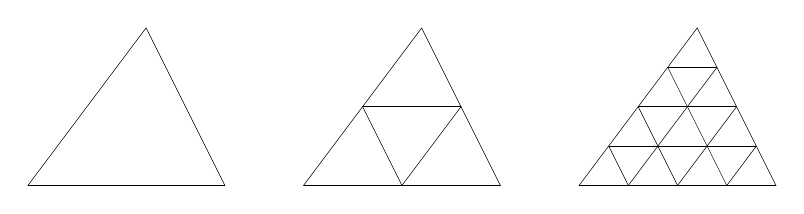
\begin{tikzpicture}
    \tkzDefPoint(-3.5,0){A''}
    \tkzDefPoint(-2,2){B''}
    \tkzDefPoint(-1,0){C''}
    \tkzDrawSegments(A'',B'' B'',C'' A'',C'')

    \tkzDefPoint(0,0){A}
    \tkzDefPoint(1.5,2){B}
    \tkzDefPoint(2.5,0){C}
    \tkzDrawSegments(A,B B,C A,C)

    \tkzDefMidPoint(A,B) \tkzGetPoint{ab}
    \tkzDefLine[orthogonal=through ab](A,B)
    \tkzDefMidPoint(A,C) \tkzGetPoint{ac}
    \tkzDefLine[orthogonal=through ac](A,C)
    \tkzDefMidPoint(B,C) \tkzGetPoint{bc}
    \tkzDefLine[orthogonal=through bc](B,C)
    \tkzDrawSegment(ab,ac)
    \tkzDrawSegment(ab,bc)
    \tkzDrawSegment(ac,bc)

    \tkzDefPoint(3.5,0){A'}
    \tkzDefPoint(5,2){B'}
    \tkzDefPoint(6,0){C'}
    \tkzDrawSegments(A',B' B',C' A',C')
    \tkzDefMidPoint(A',B') \tkzGetPoint{ab'}
    \tkzDefLine[orthogonal=through ab'](A',B')
    \tkzDefMidPoint(A',C') \tkzGetPoint{ac'}
    \tkzDefLine[orthogonal=through ac'](A',C')
    \tkzDefMidPoint(B',C') \tkzGetPoint{bc'}
    \tkzDefLine[orthogonal=through bc'](B',C')
    \tkzDrawSegment(ab',ac')
    \tkzDrawSegment(ab',bc')
    \tkzDrawSegment(ac',bc')

    \tkzDefMidPoint(A',ab') \tkzGetPoint{aab}
    \tkzDefLine[orthogonal=through aab](A',ab')
    \tkzDefMidPoint(A',ac') \tkzGetPoint{aac}
    \tkzDefLine[orthogonal=through aac](A',ac')
    \tkzDefMidPoint(ac',ab') \tkzGetPoint{x}
    \tkzDefLine[orthogonal=through x](ac',ab')
    \tkzDrawSegment(aab,aac)
    \tkzDrawSegment(aab,x)
    \tkzDrawSegment(aac,x)

    \tkzDefMidPoint(B',ab') \tkzGetPoint{abb}
    \tkzDefLine[orthogonal=through abb](B',ab')
    \tkzDefMidPoint(B',bc') \tkzGetPoint{bbc}
    \tkzDefLine[orthogonal=through bbc](B',bc')
    \tkzDefMidPoint(bc',ab') \tkzGetPoint{y}
    \tkzDefLine[orthogonal=through y](bc',ab')
    \tkzDrawSegment(abb,bbc)
    \tkzDrawSegment(abb,y)
    \tkzDrawSegment(bbc,y)

    \tkzDefMidPoint(C',ac') \tkzGetPoint{acc}
    \tkzDefLine[orthogonal=through acc](C',ac')
    \tkzDefMidPoint(C',bc') \tkzGetPoint{bcc}
    \tkzDefLine[orthogonal=through bcc](C',bc')
    \tkzDefMidPoint(bc',ac') \tkzGetPoint{z}
    \tkzDefLine[orthogonal=through z](bc',ac')
    \tkzDrawSegment(acc,bcc)
    \tkzDrawSegment(acc,z)
    \tkzDrawSegment(bcc,z)

    \tkzDefMidPoint(ab',ac') \tkzGetPoint{l}
    \tkzDefLine[orthogonal=through l](ab',ac')
    \tkzDefMidPoint(ab',bc') \tkzGetPoint{m}
    \tkzDefLine[orthogonal=through m](ab',bc')
    \tkzDefMidPoint(ac',bc') \tkzGetPoint{r}
    \tkzDefLine[orthogonal=through r](ac',bc')
    \tkzDrawSegment(l,m)
    \tkzDrawSegment(l,r)
    \tkzDrawSegment(m,r)

    \end{tikzpicture}
    \caption{Illustration of red refinement, starting with a single triangle and two successive refinement steps}
    \label{Fig3}%change all after!!!
    \end{figure}

    Let $T = [x^0, x^1, x^2]$ be the triangle to be refined, and denote $x^{ij}$ by the midpoint of the edge between $x^i$ and $x^j$.\\
    \textbf{Algorithm} Red refinement in 2D \{\\
    $T_1 := [x^0, x^{01}, x^{02}]; \qquad T_2 := [x^{01}, x^{1}, x^{12}];$\\
    $T_3 := [x^{02}, x^{12}, x^2]; \qquad T_4 := [x^{01}, x^{12}, x^{02}];$\\
    \}



    \begin{lemma*}
    Red refinement gives same congruence class in 2-dimension case.
    \end{lemma*}
    \begin{proof}\mbox{}\\
    \begin{figure}
    \centering
    \begin{tikzpicture}[scale=0.8]
    \tkzDefPoint(0,0){A}
    \tkzDefPoint(1.5,2){B}
    \tkzDefPoint(2.5,0){C}
    \tkzDrawSegments(A,B B,C A,C)

    \tkzLabelPoints[above,yshift=0pt](B)
    \tkzLabelPoints[left,yshift=4pt](A)
    \tkzLabelPoints[right,yshift=4pt](C)
    \tkzDefMidPoint(A,B) \tkzGetPoint{X}
    \tkzDefLine[orthogonal=through ab](A,B)
    \tkzDefMidPoint(A,C) \tkzGetPoint{Z}
    \tkzDefLine[orthogonal=through ac](A,C)
    \tkzDefMidPoint(B,C) \tkzGetPoint{Y}
    \tkzDefLine[orthogonal=through bc](B,C)
    \tkzDrawSegment(X,Z)
    \tkzDrawSegment(X,Y)
    \tkzDrawSegment(Z,Y)
    \tkzLabelPoints[above,xshift=-2mm](X)
    \tkzLabelPoints[above,xshift=2mm](Y)
    \tkzLabelPoints[below](Z)
    \end{tikzpicture}
    \caption{Illustration of Uniform Refinement for the Lemma}
    \label{Fig4}
    \end{figure}

    Let A, B, C be the vertices of the triangle $T$ and let X, Y, Z be the midpoints of the edge AB, BC and AC. An application of red refinement produces the triangle $T_1 = [A, X, Z]$, $T_2 = [X, B, Y]$, $T_3 = [Z, Y, C]$ and $T_4 = [Y, Z, X]$. Consider the picture above.

    We have line XY parallel to line AC, i.e., $XY \parallel AC$, so $\angle{BXY} = \angle{XAZ}$. Similarily, since $XZ\parallel BC$, we have $\angle{XBY} = \angle{AXZ}$. Since X is the midpoint of line AB, then $|AX| = |BX|$. In short, we have 
    \begin{align*}
    \angle{BXY} = \angle{XAZ},
    \quad
    |BX| = |AX|,
    \quad
    \angle{XBY} = \angle{AXZ}.
    \end{align*}
    Therefore, $\triangle{BXY} \cong \triangle{XAZ}$. Similarily, we can prove the four triangles are congruent to each other, i.e., $\triangle{BXY}\cong\triangle{XAZ}\cong\triangle{YZC} \cong\triangle{ZYX}$, so they are in a same congruent class, which is same as the one of the original triangle $\triangle{BAC}$.
    \end{proof}
    By the lemma above, we know that red refinement applied on a non degenerate simplex in 2 dimension gives one congruent class. Moreover, by Theorem in 3.1, we see that red refinement strategy is stable.
    [This lemma leads to stability]

    \begin{lemma*}
    Red refinement preserves consistency in the 2-dimensional case.
    \end{lemma*}
    %\begin{proof}\mbox{}\\
    %This is obvious as how simplicial complex is defined.
    %\end{proof}

    %\paragraph{Stability and Consistency}\mbox{}\\
    \subsection{Stability and Consistency}
    Subdividing a triangle by connecting its midpoint, we obtain four congruent simplices $T_1, T_2, T_3$ and $T_4$. The green refinement, an irregular refinement which connects the refined edge midpoint to its opposite corner, is applied on one refined edge on which we may confront with degenerate simplices. We will never touch and refine such simplices to avoid them from degenerating.

    Clearly, the red refinement strategy is stable since it produces a finite number of triangles congruent to the original simplex. Meanwhile, we preserve consistency by bisecting triangles with one refined edge and never refine them any further. Therefore, we obtain stability and consistency through red and green refinement.

    %\paragraph{Vertices and Edges by Red Refinement in 2D}\mbox{}\\
    \subsection{Counting Vertices and Edges by Red Refinement in 2D}
    In Figure 2 above, we see that we obtain four congruent triangles similar to the original large triangle. Lemma 1 below presents relationship between number of triangles and number of times that red refinement is applied.

    \begin{lemma}
    Denote $T_{m}$ as the number of triangles after applying red refinement m times, then,
    \begin{align*}
    T_{m+1} = 4 \cdot T_{m}, \quad T_{m} = 4^m \cdot T_0
    \end{align*}
    \end{lemma}
    \begin{proof}
    Based on Figure 3, we see that we always obtain 4 similar triangles that is same as the original one. In other words, we have $T_{m+1} = 4 \cdot T_{m}$.\\
    To prove $T_{m} = 4^m \cdot T_0$ by induction, we have the base case that $T_1 = 4^1 \cdot T_0$ in Figure 3. Suppose that this is true for $T_{m} = 4^m \cdot T_0$, we need to prove this holds true for $T_{m+1}$.\\
    Since we have $T_{m+1} = 4 \cdot T_{m}$, and by inductive hypothesis, we have
    \begin{align*}
    T_{m+1} = 4 \cdot T_{m} = 4 \cdot (4^m\cdot T_0) = 4^{m+1}\cdot T_0
    \end{align*}
    Therefore, by induction, we proved that $T_{m+1} = 4 \cdot T_{m}$.
    \end{proof}

    \begin{lemma}
    Denote $E_{m}$ as the number of edges of a simplicial complex $\mathcal{T}$ obtained by applying red refinement m times, then,
    \begin{align*}
    E_{m+1} = 2 \cdot E_m + 3 \cdot T_m, \quad E_{m} = 2^{m}\cdot E_0 + 3 \cdot2^{m-1}\cdot(2^{m} -1)\cdot T_0
    \end{align*}
    \end{lemma}
    \begin{proof}
    After applying the red refinement one more time, that is m+1 times in total, then we can think like in each smaller triangle in $T_m$, we again have double number of edges by bisecting edges, and obtain number of $T_m$ edges from connecting each midpoints. Therefore, we have $E_{m+1} = 2\cdot E_m + 3\cdot T_m$.\\
    The proof of the latter part can also be done by induction. The base case is obvious by Figure 3, that is $E_1 = 9 = 2^1\cdot 3 + 3\cdot 2^0 \cdot (2^1 - 1)\cdot1 = 2^1\cdot E_0 + 3\cdot2^{1-1}\cdot(2^1 - 1)\cdot T_0$.\\
    Suppose that this holds after applying red refinement m times, i.e., $E_{m} = 2^{m} E_0 + 3 \cdot2^{m-1}\cdot(2^{m} -1)\cdot T_0$. Since $E_{m+1} = 2 \cdot E_m + 3 \cdot T_m$, and by the inductive hypothesis and Lemma 1, we have
    \begin{align*}
    E_{m+1} &= 2 \cdot E_m + 3 \cdot T_m \\
    &= 2(2^{m}\cdot E_0 + 3 \cdot2^{m-1}\cdot(2^{m} -1)\cdot T_0) + 3\cdot 4^m\cdot T_0\\
    &= 2^{m+1}\cdot E_0 + 3\cdot2^m\cdot(2^m - 1)\cdot T_0 + 3\cdot4^m\cdot T_0\\
    &= 2^{m+1}\cdot E_0 + 3\cdot(2^m\cdot(2^m -1 + 2^m))\cdot T_0\\
    &=2^{m+1}\cdot E_0 + 3\cdot2^m\cdot(2^{m+1}-1)\cdot T_0
    \end{align*}
    Thus, we finished the proof by induction.
    \end{proof}

    \begin{lemma}
    Denote $V_{m}$ as the number of vertices of a simplicial complex $\mathcal{T}$ obtained by applying red refinement m times, then,
    \begin{align*}
    V_{m+1} = V_{m} + E_{m}, \quad V_m = V_0 + (2^m -1)\cdot E_0 + (2^{m-1}\cdot(2^m+3)-2)\cdot T_0
    \end{align*}
    \end{lemma}
    \begin{proof}
    Whenever red refinement is applied, we set a midpoint on each edge as a new vertex. That is, we obtain a same number of new vertices as the number of edges of the simplicial complex before applying the red refinement. After applying the red refinement one more time, the number of new vertices is same as the number of edges of $T_m$, i.e., $E_m$. Then adding together, we have $V_{m+1} = V_m + E_m$.\\
    Suppose that $V_m = V_0 + (2^m -1)\cdot E_0 + (2^{m-1} -1)(2^m -1)\cdot T_0$. Then by Lemma 2, we have
    \begin{align*}
    V_{m+1} &= V_m + E_m\\
    &= V_m + 2^m\cdot E_0 + 3\cdot 2^{m-1}\cdot(2^m-1)\cdot T_0\\
    &= V_0 + \sum_{k=0}^m 2^k E_0 + 3\cdot 2^{k-1}\cdot(2^k-1)\cdot T_0\\
    &= V_0 + \sum_{k=0}^m 2^k E_0 + 3\sum_{k=0}^m 2^{2k-1}\cdot T_0 + 3\sum_{k=0}^m 2^{k-1}\cdot T_0\\
    &= V_0 + (2^{m+1}-1)E_0 + \frac{3}{2}\sum_{k=0}^m 4^k\cdot T_0 + \frac{3}{2}\sum_{k=0}^m 2^k\cdot T_0\\
    &= V_0 + (2^{m+1}-1)E_0 + \frac{3}{2}\cdot\frac{4^{m+1}-1}{3}\cdot T_0 + \frac{3}{2}(2^{m+1}-1)\cdot T_0\\
    &= V_0 + (2^{m+1}-1)E_0 + \frac{4^{m+1}-1 + 3\cdot2^{m+1} -3}{2}\cdot T_0\\
    &= V_0 + (2^{m+1}-1)E_0 + (2^m\cdot(2^{m+1}+3)-2)\cdot T_0
    \end{align*}
    Thus, we finished the proof.
    \end{proof}


    %\subsection{3D}

  \section{Bisection}
        \subsection{Newest Vertex Bisection Refinement in 2-dimension and its stability}
    Another popular refinement strategy is bisection. Basically, we cut a triangle by connecting one vertex, which we choose as the peak, with its opposite edge, which we call refinement edge. Generally, if we apply random bisection with no plan on a triangle, it is likely that we fail to preserve stability and consistency.

    Hence, one important part we need to consider is how to choose the peak for a triangle to preserve the stability and consistency, and one famous method was introduced as the $newest vertex$ bisection. In newest vertex bisection, we create the newest vertex at the middle of the refinement edge after applying the bisection refinement once, and then we regard the newest vertex as the peak for bisection over the resulting two smaller triangles.

    \begin{figure}[h!]
    \centering
    \captionsetup{justification=centering}
      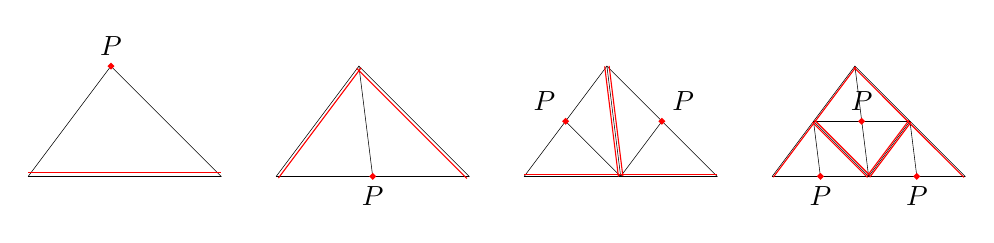
\begin{tikzpicture}[scale=0.7]

      %use to draw parallel line
      \tikzset{
      ncbar/.style={
        to path=%
        ($(\tikztostart)!#1!90:(\tikztotarget)$)
        -- ($(\tikztotarget)!($(\tikztostart)!#1!90:(\tikztotarget)$)!90:(\tikztostart)$)
      },
      ncbar/.default=0.2,
      }

      %triangle#1
      \tkzDefPoint(-6.5,0){A''}
      \tkzDefPoint(-5,2){B''}
      \tkzDefPoint(-3,0){C''}
      \tkzDrawSegments(A'',B'' B'',C'' A'',C'')
      %peak
      \fill[red!20, draw=red, thick] (B'') circle (1pt) node[black, above] {$P$};
      %refinement edge
      \draw[red] (A'') to[ncbar=0.02] (C'');

      %triangle#2
      \tkzDefPoint(-2,0){A}
      \tkzDefPoint(-0.5,2){B}
      \tkzDefPoint(1.5,0){C}
      \tkzDrawSegments(A,B B,C A,C)

      \tkzDefMidPoint(A,C) \tkzGetPoint{ac}
      \tkzDefLine[orthogonal=through ac](A,C)
      \tkzDrawSegment(B,ac)
      %peak
      \fill[red!20, draw=red, thick] (ac) circle (1pt) node[black, below] {$P$};
      %refinement edge1
      \draw[red] (A) to[ncbar=-0.02] (B);
      %refinement edge2
      \draw[red] (B) to[ncbar=-0.02] (C);

      %triangle#3
      \tkzDefPoint(2.5,0){A'}
      \tkzDefPoint(4,2){B'}
      \tkzDefPoint(6,0){C'}
      \tkzDrawSegments(A',B' B',C' A',C')
      \tkzDefMidPoint(A',B') \tkzGetPoint{ab'}
      \tkzDefLine[orthogonal=through ab'](A',B')
      \tkzDefMidPoint(A',C') \tkzGetPoint{ac'}
      \tkzDefLine[orthogonal=through ac'](A',C')
      \tkzDefMidPoint(B',C') \tkzGetPoint{bc'}
      \tkzDefLine[orthogonal=through bc'](B',C')
      \tkzDrawSegment(B',ac')
      \tkzDrawSegment(ac',ab')
      \tkzDrawSegment(ac',bc')

      %peak1
      \fill[red!20, draw=red, thick] (ab') circle (1pt) node[black, above left] {$P$};
      %peak2
      \fill[red!20, draw=red, thick] (bc') circle (1pt) node[black, above right] {$P$};
      %refinement edges
      \draw[red] (A') to[ncbar=0.02] (ac');
      \draw[red] (C') to[ncbar=-0.02] (ac');
      \draw[red] (B') to[ncbar=0.02] (ac');
      \draw[red] (B') to[ncbar=-0.02] (ac');


      %triangle#4
      \tkzDefPoint(7,0){A'''}
      \tkzDefPoint(8.5,2){B'''}
      \tkzDefPoint(10.5,0){C'''}
      \tkzDrawSegments(A''',B''' B''',C''' A''',C''')
      \tkzDefMidPoint(A''',B''') \tkzGetPoint{ab''}
      \tkzDefLine[orthogonal=through ab''](A''',B''')
      \tkzDefMidPoint(A''',C''') \tkzGetPoint{ac''}
      \tkzDefLine[orthogonal=through ac''](A''',C''')
      \tkzDefMidPoint(B''',C''') \tkzGetPoint{bc''}
      \tkzDefLine[orthogonal=through bc''](B''',C''')
      \tkzDrawSegment(B''',ac'')
      \tkzDrawSegment(ac'',ab'')
      \tkzDrawSegment(ac'',bc'')
      \tkzDefMidPoint(B''',ac'') \tkzGetPoint{x}
      \tkzDefLine[orthogonal=through x](B''',ac'')
      \tkzDefMidPoint(A''',ac'') \tkzGetPoint{y}
      \tkzDefLine[orthogonal=through y](A''',ac'')
      \tkzDefMidPoint(C''',ac'') \tkzGetPoint{z}
      \tkzDefLine[orthogonal=through z](C''',ac'')
      \tkzDrawSegment(ab'',x)
      \tkzDrawSegment(bc'',x)
      \tkzDrawSegment(ab'',y)
      \tkzDrawSegment(bc'',z)

      %peaks
      \fill[red!20, draw=red, thick] (x) circle (1pt) node[black, above] {$P$};
      \fill[red!20, draw=red, thick] (y) circle (1pt) node[black, below] {$P$};
      \fill[red!20, draw=red, thick] (z) circle (1pt) node[black, below] {$P$};

      %refinement edges
      \draw[red] (A''') to[ncbar=-0.02] (ab'');
      \draw[red] (ab'') to[ncbar=-0.02] (ac'');
      \draw[red] (bc'') to[ncbar=-0.02] (C''');
      \draw[red] (bc'') to[ncbar=0.02] (ac'');
      \draw[red] (B''') to[ncbar=0.02] (ab'');
      \draw[red] (ab'') to[ncbar=0.02] (ac'');
      \draw[red] (bc'') to[ncbar=-0.02] (ac'');
      \draw[red] (B''') to[ncbar=-0.02] (bc'');
    \end{tikzpicture}
    \caption{Illustration of bisection refinement, starting with a single triangle\\P represents a peak, and red line denotes a refinement edge}
    \label{Fig5}
    \end{figure}







%----------------------------------------------------------------------------------
    %\subsection{Stability of Newest Vertex Bisection}
    \begin{lemma*}
    Bisection refinement gives four congruence classes given one triangle.
    \end{lemma*}
    \begin{proof}
    \begin{figure}[h!]
    \centering
    \captionsetup{justification=centering}
      \begin{tikzpicture}[scale=0.8]
      %use to draw parallel line
      \tikzset{
      ncbar/.style={
        to path=%
        ($(\tikztostart)!#1!90:(\tikztotarget)$)
        -- ($(\tikztotarget)!($(\tikztostart)!#1!90:(\tikztotarget)$)!90:(\tikztostart)$)
      },
      ncbar/.default=0.2,
      }

      %Stage 1 - Triangle
      \tkzDefPoint(-9,0){A''}
      \tkzDefPoint(-7.5,2){B''}
      \tkzDefPoint(-5.5,0){C''}
      \tkzDrawSegments(A'',B'' B'',C'' A'',C'')
      \node (t) at (-7.5, 1) {{1}};
      %peaks
      \fill[red!20, draw=red, thick] (B'') circle (1pt) node[black, above] {$P$};
      %refinement edge
      \draw[red] (A'') to[ncbar=0.02] (C'');

      %Stage 2 - Triangle
      \tkzDefPoint(-2,0){A}
      \tkzDefPoint(-0.5,2){B}
      \tkzDefPoint(1.5,0){C}
      \tkzDrawSegments(A,B B,C A,C)
      \tkzDefMidPoint(A,C) \tkzGetPoint{ac}
      \tkzDefLine[orthogonal=through ac](A,C)
      \tkzDrawSegment(B,ac)
      \node (t') at (-1, 0.5) {{2}};
      \node (t'') at (0.5, 0.5) {{3}};
      %peaks
      \fill[red!20, draw=red, thick] (ac) circle (1pt) node[black, below] {$P$};
      %refinement edge
      \draw[red] (A) to[ncbar=-0.02] (B);
      \draw[red] (B) to[ncbar=-0.02] (C);
      \end{tikzpicture}
    \caption{Stage 1: Original triangle(left) in congruence class 1\\Stage 2: Applied the newest vertex bisection once(right) in congruence class 2 and 3}
    \label{fig6: sub1}
    \end{figure}

    Observing \ref{fig6: sub1}, we have a triangle at the beginning, say it's in congruency class 1. After applying the newest vertex bisection refinement once, see \ref{fig6: sub1}, we obtain two smaller pieces of triangles as in the second picture in Figure 5. Say one of them is in congruency class 2, and another one is in congruency class 3. Further applying the newest vertex bisection refinement, we have the triangulation in \ref{fig6: sub2}.

    \begin{figure}[h!]
    \centering
    \captionsetup{justification=centering}
      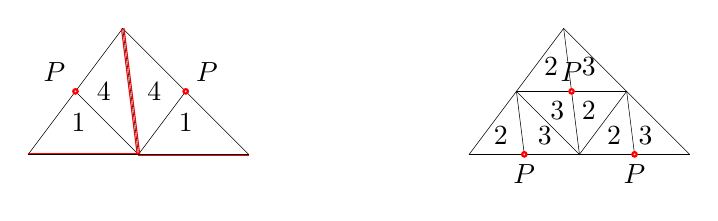
\begin{tikzpicture}[scale=0.8] 
      %use to draw parallel line
      \tikzset{
      ncbar/.style={
        to path=%
        ($(\tikztostart)!#1!90:(\tikztotarget)$)
        -- ($(\tikztotarget)!($(\tikztostart)!#1!90:(\tikztotarget)$)!90:(\tikztostart)$)
      },
      ncbar/.default=0.2,
      }

      %Stage 3 - Triangle
      \tkzDefPoint(0,0){A'}
      \tkzDefPoint(1.5,2){B'}
      \tkzDefPoint(3.5,0){C'}
      \tkzDrawSegments(A',B' B',C' A',C')
      \tkzDefMidPoint(A',B') \tkzGetPoint{ab'}
      \tkzDefLine[orthogonal=through ab'](A',B')
      \tkzDefMidPoint(A',C') \tkzGetPoint{ac'}
      \tkzDefLine[orthogonal=through ac'](A',C')
      \tkzDefMidPoint(B',C') \tkzGetPoint{bc'}
      \tkzDefLine[orthogonal=through bc'](B',C')
      \tkzDrawSegment(B',ac')
      \tkzDrawSegment(ac',ab')
      \tkzDrawSegment(ac',bc')
      \node (t''') at (1.2, 1) {{4}};
      \node (t''') at (2, 1) {{4}};
      \node (t) at (0.8, 0.5) {{1}};
      \node (t) at (2.5, 0.5) {{1}};
      %peaks
      \fill[red!20, draw=red, thick] (ab') circle (1pt) node[black, above left] {$P$};
      %refinement edge
      \draw[red] (A') to[ncbar=0.01] (ac');
      \draw[red] (B') to[ncbar=-0.01] (ac');
      %peaks
      \fill[red!20, draw=red, thick] (bc') circle (1pt) node[black, above right] {$P$};
      %refinement edge
      \draw[red] (C') to[ncbar=0.01] (ac');
      \draw[red] (B') to[ncbar=0.01] (ac');

      %Stage 4 - Triangle
      \tkzDefPoint(7,0){A'''}
      \tkzDefPoint(8.5,2){B'''}
      \tkzDefPoint(10.5,0){C'''}
      \tkzDrawSegments(A''',B''' B''',C''' A''',C''')
      \tkzDefMidPoint(A''',B''') \tkzGetPoint{ab''}
      \tkzDefLine[orthogonal=through ab''](A''',B''')
      \tkzDefMidPoint(A''',C''') \tkzGetPoint{ac''}
      \tkzDefLine[orthogonal=through ac''](A''',C''')
      \tkzDefMidPoint(B''',C''') \tkzGetPoint{bc''}
      \tkzDefLine[orthogonal=through bc''](B''',C''')
      \tkzDrawSegment(B''',ac'')
      \tkzDrawSegment(ac'',ab'')
      \tkzDrawSegment(ac'',bc'')
      \tkzDefMidPoint(B''',ac'') \tkzGetPoint{x}
      \tkzDefLine[orthogonal=through x](B''',ac'')
      \tkzDefMidPoint(A''',ac'') \tkzGetPoint{y}
      \tkzDefLine[orthogonal=through y](A''',ac'')
      \tkzDefMidPoint(C''',ac'') \tkzGetPoint{z}
      \tkzDefLine[orthogonal=through z](C''',ac'')
      \tkzDrawSegment(ab'',x)
      \tkzDrawSegment(bc'',x)
      \tkzDrawSegment(ab'',y)
      \tkzDrawSegment(bc'',z)
      \node (t') at (7.5, 0.3) {{2}};
      \node (t'') at (8.2, 0.3) {{3}};
      \node (t'') at (8.4, 0.7) {{3}};
      \node (t') at (8.3, 1.4) {{2}};
      \node (t'') at (8.9, 1.4) {{3}};
      \node (t') at (8.9, 0.7) {{2}};
      \node (t') at (9.3, 0.3) {{2}};
      \node (t'') at (9.8, 0.3) {{3}};
      %peaks
      \fill[red!20, draw=red, thick] (x) circle (1pt) node[black, above] {$P$};
      \fill[red!20, draw=red, thick] (y) circle (1pt) node[black, below] {$P$};
      \fill[red!20, draw=red, thick] (z) circle (1pt) node[black, below] {$P$};
      %refinement edge need???
      
      \end{tikzpicture}
    \caption{Stage 3: Applied the newest vertex bisection twice(left) in congruence class 1 and 4\\Stage 4: Applied the newest vertex bisection three times(right) in congruence class 2 and 3}
    \label{fig6: sub2}
    \end{figure}

    \begin{claim}
    The left and right bottom triangles in Stage 3 are congruent to the original triangle in Stage 1, and they are in the congruency class 1. Moreover, the other two triangles left are congruent and in congruency class 4.
    \end{claim}
    %\begin{proof}\mbox{}\\
    \noindent
    Proof of Claim 1: \\
    Let A, B, C be the vertices of the triangle $T$ and let X, Y, Z be the midpoints of the edge AB, AC and BC. An application of the newest vertex bisection refinement produces the triangle $\triangle{AXY}, \triangle{XBY}, \triangle{ZBY}$ and $\triangle{YZC}$. Consider the Fig 8 (left).
    Since X, Y, Z be the midpoints of the edge AB, AC and BC, we have 
    \begin{align*}
     XY \parallel BC,
     \quad 
     ZY \parallel AB,
     \quad 
     AX = BX, 
     \quad 
     BZ = CZ, 
     \quad
     AY = CY
    \end{align*}
    Since $XY\parallel BC$, we have $\angle{AXY} = \angle{ABC}$ and $\angle{XYB} = \angle{ZBY}$. Similarly, since $ZY\parallel AB$, we have $\angle{YZC} = \angle{ABC}$ and $\angle{XBY} = \angle{ZYB}$. Thus 
    \begin{align*}
    \angle{XYB} = \angle{ZBY},
    \quad
    |BY| = |BY|,
    \quad
    \angle{XBY} &= \angle{ZYB}.
    \end{align*}
    Therefore, we have $\triangle{XBY} \cong \triangle{ZYB}$, and we mark them in the congruency class 4. This further gives us $|AX| = |BX| = |YZ|$, and $|ZC| = |BZ| = |XY|$.
    \begin{align*}
    |AX| = |YZ|,
    \quad
    \angle{AXY} = \angle{ABC} = {YZC},
    \quad
    |XY| = |ZC|.
    \end{align*}
    Therefore, we have $\triangle{AXY} \cong \triangle{YZC}$. It's clear that $\triangle{AXY}$ and $\triangle{YZC}$ are similar to $\triangle{ABC}$ as all their angles are the same. Thus, we finished the proof of claim 1.

    %\end{proof}%end proof of claim 1

    \begin{claim}
    Triangles with same number in Stage 4 in a same congruency class marked by the number.
    \end{claim}
    %\begin{proof}
    \noindent
    Proof of Claim 2: \\
    Let A, B, C be the vertices of the triangle $T$ and let X, Y, Z be the midpoints of the edge AB, AC and BC, and M, N, P be the midpoints of the edge AY, CY and BY. Consider the Fig 8 (right).
 
    An application of the newest vertex bisection refinement produces the following triangles
    \begin{align*}
    \triangle{AXM}, \triangle{XBP}, \triangle{ZYP}, \triangle{YZN}, \triangle{MXY}, \triangle{PBZ}, \triangle{PYX}, \triangle{NZC}
    \end{align*}
    Notice that X, P and Z are three points one a stright line. This is clear because $XP\parallel AY$ and $PZ\parallel YC$, and we have $\angle{BPX}+\angle{BPZ} = \angle{BYA}+\angle{BYC} = \pi$. Basically, to prove the Stage 4 is equivalent to prove the following
    \begin{align*}
    \triangle{AXM}\cong\triangle{XBP}\cong\triangle{ZYP}\cong\triangle{YZN}\\
    \triangle{MXY}\cong\triangle{PBZ}\cong\triangle{PYX}\cong\triangle{NZC}
    \end{align*}
    Similarily to proof of Claim 1, we have
    \begin{align*}
    XY\parallel BC,
    \quad
    YZ\parallel AB,
    \quad
    XZ\parallel AC,
    \quad
    XM\parallel BY\parallel ZN
    \end{align*}
    Therefore, we further have 
    \begin{align*}
    \angle{BAY} = \angle{ZYC},
    \quad
    \angle{BCY} = \angle{XYA},
    \quad
    \angle{AXC} = \angle{ABC} = \angle{YZC}\\
    \angle{PZY} = \angle{ZYN},
    \quad
    \angle{PYZ} = \angle{NZP},
    \quad
    \angle{PXY} = \angle{XYM},
    \quad
    \angle{PYX} = \angle{MXY},
    \end{align*}
    Then it is clear that
    \begin{align*}
    \triangle{AXY} \sim \triangle{ABC} \sim \triangle{YZC}
    \end{align*}
    Similarly, we can find that 
    \begin{align*}
    \triangle{XBZ}\sim\triangle{ABC},
    \quad
    \triangle{AXM}\sim\triangle{ABY},
    \quad
    \triangle{CZN}\sim\triangle{CBY}.
    \end{align*}
    In other words, 
    \begin{align*}
    \triangle{AXM}\sim\triangle{ABY}\sim\triangle{XBP}\sim\triangle{YZN},\\
    \triangle{CZN}\sim\triangle{CBY}\sim\triangle{YXM}\sim\triangle{ZBP}.
    \end{align*}
    Moreover, since the ratio of $\|AX\|, \|BX\|$, and $\|ZY\|$ is 1, and the ratio of $\|ZC\|, \|BZ\|$, and $\|XY\|$ is 1, we have
    \begin{align*}
    \triangle{AXM}\cong\triangle{XBP}\cong\triangle{YZN},\\
    \triangle{CZN}\cong\triangle{YXM}\sim\triangle{ZBP}.
    \end{align*}
    Therefore, we showed that $\triangle{AXM}, \triangle{XBP}$ and $\triangle{YZN}$ are in congruency class 2, and $\triangle{CZN}, \triangle{YXM}$ and $\triangle{ZBP}$ are in congruency class 3.
    Moreover, since 
    \begin{align*}
    \angle{PZY} = \angle{ZYN},
    \quad
    \angle{PYZ} = \angle{NZP},
    \quad
    \angle{PXY} = \angle{XYM},
    \quad
    \angle{PYX} = \angle{MXY},
    \end{align*}
    we have that
    \begin{align*}
    \triangle{YZN}\cong\triangle{YZP},
    \quad
    \triangle{YXM}\cong\triangle{YXP}.
    \end{align*}
    Therefore we proved 
    \begin{align*}
    \triangle{AXM}\cong\triangle{XBP}\cong\triangle{ZYP}\cong\triangle{YZN}\sim\triangle{ABY},\\
    \triangle{MXY}\cong\triangle{PBZ}\cong\triangle{PYX}\cong\triangle{NZC}\sim\triangle{YBC}.
    \end{align*}
    %\end{proof}
    Thus, we finished proof of Claim 2.
    
    %------------------------------------------------------------------------
    %figure for claims proof
    \begin{figure}[h!]
    \centering
    \captionsetup{justification=centering}
    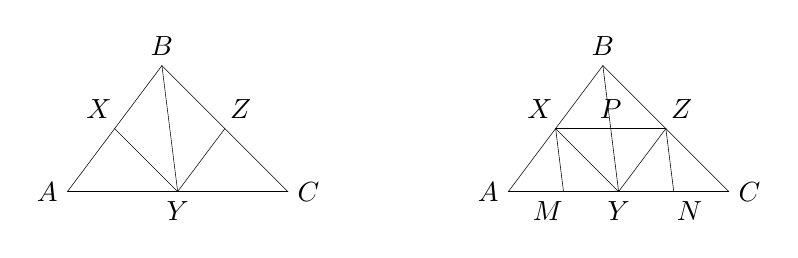
\begin{tikzpicture}[scale=0.8]
    \tkzDefPoint(-4.5,0){A}
    \tkzDefPoint(-3,2){B}
    \tkzDefPoint(-1,0){C}
    \tkzDrawSegments(A,B B,C A,C)
    \tkzLabelPoints[left](A)
    \tkzLabelPoints[above](B)
    \tkzLabelPoints[right](C)
    \tkzDefMidPoint(A,B) \tkzGetPoint{X}
    \tkzDefLine[orthogonal=through X](A,B)
    \tkzDefMidPoint(A,C) \tkzGetPoint{Y}
    \tkzDefLine[orthogonal=through Y](A,C)
    \tkzDefMidPoint(B,C) \tkzGetPoint{Z}
    \tkzDefLine[orthogonal=through Z](B,C)
    \tkzDrawSegment(B,Y)
    \tkzDrawSegment(Y,X)
    \tkzDrawSegment(Y,Z)
    \tkzLabelPoints[above, xshift=-2mm](X)
    \tkzLabelPoints[above, xshift=2mm](Z)
    \tkzLabelPoints[below,yshift=0pt](Y)

    \tkzDefPoint(2.5,0){A}
    \tkzDefPoint(4,2){B}
    \tkzDefPoint(6,0){C}
    \tkzDrawSegments(A,B B,C A,C)
    \tkzLabelPoints[left](A)
    \tkzLabelPoints[above](B)
    \tkzLabelPoints[right](C)
    \tkzDefMidPoint(A,B) \tkzGetPoint{X}
    \tkzDefLine[orthogonal=through X](A,B)
    \tkzDefMidPoint(A,C) \tkzGetPoint{Y}
    \tkzDefLine[orthogonal=through Y](A,C)
    \tkzDefMidPoint(B,C) \tkzGetPoint{Z}
    \tkzDefLine[orthogonal=through Z](B,C)
    \tkzDrawSegment(B,Y)
    \tkzDrawSegment(Y,X)
    \tkzDrawSegment(Y,Z)
    \tkzLabelPoints[above, xshift=-2mm](X)
    \tkzLabelPoints[above, xshift=2mm](Z)
    \tkzLabelPoints[below,yshift=0pt](Y)

    \tkzDefMidPoint(B,Y) \tkzGetPoint{P}
      \tkzDefLine[orthogonal=through P](B,Y)
      \tkzDefMidPoint(A,Y) \tkzGetPoint{M}
      \tkzDefLine[orthogonal=through M](A,Y)
      \tkzDefMidPoint(C,Y) \tkzGetPoint{N}
      \tkzDefLine[orthogonal=through N](C,Y)
      \tkzDrawSegment(X,P)
      \tkzDrawSegment(Z,P)
      \tkzDrawSegment(X,M)
      \tkzDrawSegment(Z,N)
      \tkzLabelPoints[below, xshift=-2mm](M)
    \tkzLabelPoints[below, xshift=2mm](N)
    \tkzLabelPoints[above,yshift=0pt](P)
    \end{tikzpicture}
    \caption{Illustration of newest vertex bisection for Claim 1(left); Claim 2(right)}
    \label{Fig8}
    \end{figure}



    Notice that in Stage 3, we see triangles in congruency class 1 again, so we can tell further applying the newest vertex bisection refinement will lead to the same process as what we have for Stage 1. Similarly, further applying the newest vertex bisection refinement over triangles in congruency class 4, 2 and 3 are already explored in Stage 3 and 4. Therefore, we actually obtain 4 congruency classes only.
    \end{proof}
    This means that we never have triangles degenerating when applying the newest vertex bisection refinement, because the number of congruence classes is four, which is finite, and by theorem proved in 3.1, we see that the newest vertex bisection refinement strategy is stable.

    As we explain in section 3, a good refinement strategy should preserve both stability and consistency. Before we take a look at consistency, let's first introduce dependency graph.

    \subsection{Compatible Divisibility and Consistency}
    \begin{definition*}
      Let G = (N, A) be a simple directed graph, where N(nodes) represents triangles, and $(n_1, n_2)\in A (arrows)$ if the refinement edge of $n_1$ neighbors at $n_2$, and then we call G a dependency graph.
      \begin{align*}
      N &= \{T\in\mathcal{T}~\mid~\diam{T} = 2\}\\
      A &= \{(V_1, V_2)\in V\times V | \text{The refinement edge of $V_1$ neighbors $V_2$}\}
      \end{align*}
    \end{definition*}
    Note that $G$ is a simple directed graph, so it does not contain any loops. That is, for all $(v_1, v_2)\in A$, we have $v_1\neq v_2$. Moreover, all nodes of one dependency graph have at most one outgoing arrow, because every triangle $T$ has at most exactly one refinement edge(See \ref{Fig9}). If the refinement edge of $T$ borders no other triangles, then there is no arrow going from $T$ to any other triangles in the dependency graph. If oppositely, it borders another triangle $T'$ along its refinement edge, then there is an arrow in G going from $T$ to $T'$.  %[Multiple V's, graph? need proof???]
    \begin{figure}[h!]
    \centering
    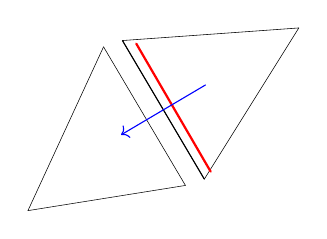
\begin{tikzpicture}[scale=0.8]
    \tkzDefPoint(0.5,0.1){A}
    \tkzDefPoint(3,0.5){B}
    \tkzDefPoint(1.7,2.7){C}
    \tkzDrawSegments(A,B B,C A,C)

    \tkzDefPoint(2,2.8){A'}
    \tkzDefPoint(3.3,0.6){B'}
    \tkzDefPoint(4.8,3){C'}
    \tkzDrawSegments(A',B' B',C' A',C')

    \tkzDefPoint(2.22,2.75){X}
    \tkzDefPoint(3.4,0.72){Y}
    \tkzDrawSegment[thick, color=red](X, Y)
    \draw (A') -- (B') node[pos=0.5, sloped] (mid){};
    \draw[->,shorten >=-0.5cm, shorten <=-0.5cm, blue] (mid.north)--(mid.south);
    %\draw [blue,  ->   ] (3.35,2.2) -- (1.2,0.7);
    \end{tikzpicture}
    \caption{Illustration of outgoing arrow in dependency graph}
    \label{Fig9}
    \end{figure}

    \begin{lemma*}
    A node n in the dependency graph has no outgoing arrow if and only if the corresponding triangle of n has a refinement edge at the boundary.
    \end{lemma*}
    The proof for this is trivial based on the explanation for G as simple graph.

    \begin{definition*}
      A triangle is called compatibly divisible if either
      \begin{itemize}
        \item[a. ] it has no outgoing edge in G
        \item[b. ] it is part of a cycle in G whose size is 2.
      \end{itemize}
    \end{definition*}
    \begin{figure}[h!]
    \centering
    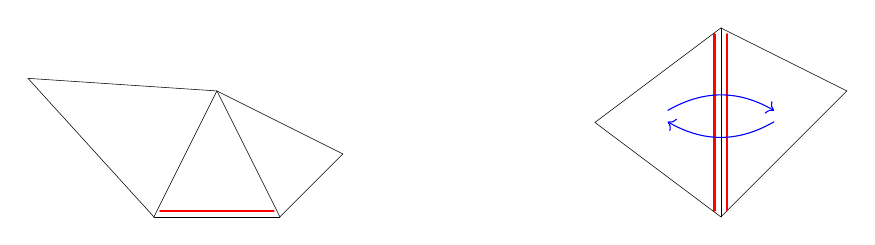
\begin{tikzpicture}[scale=0.8]
    \tkzDefPoint(-4,0){A}
    \tkzDefPoint(-3,2){B}
    \tkzDefPoint(-2,0){C}
    \tkzDrawSegments(A,B B,C A,C)
    \tkzDefPoint(-6,2.2){D}
    \tkzDrawSegments(A,D B,D)
    \tkzDefPoint(-1,1){E}
    \tkzDrawSegments(C,E B,E)
    %\tkzDefPoint(-5,0.5){F}
    %\tkzDrawSegments(A,F)
    %\tkzDefPoint(-1.5,0){G}
    %\tkzDrawSegments(C,G)
    \tkzDefPoint(-3.9,0.1){X}
    \tkzDefPoint(-2.1,0.1){Y}
    \tkzDrawSegment[thick, color=red](X, Y)

    \tkzDefPoint(3,1.5){A'}
    \tkzDefPoint(5,0){B'}
    \tkzDefPoint(5,3){C'}
    \tkzDrawSegments(A',B' B',C' A',C')
    \tkzDefPoint(7,2){D'}
    \tkzDrawSegments(B',D' C',D')
    \tkzDefPoint(4.9,0.1){X'}
    \tkzDefPoint(4.9,2.9){Y'}
    \tkzDefPoint(5.1,0.1){M'}
    \tkzDefPoint(5.1,2.9){N'}
    \tkzDrawSegment[thick, color=red](X', Y')
    \tkzDrawSegment[thick, color=red](M', N')

    \node (b) at (6, 1.6){};
    \node (a) at (4, 1.6){}
       edge [<-, blue, bend right=30] (b)
       ;
    \node (b) at (6, 1.6){}
       edge [<-, blue, bend right=30] (a)
       ;

    %\draw [->, blue] (4, 1.6) to [out=50,in=2] (6, 1.6);
    %\draw [->, blue] (6, 1.4) to [out=-20,in=-2] (4, 1.4);
    \end{tikzpicture}
    \caption{Compatibly divisible triangles: case a(left); case b(right)}
    \label{Fig10}
    \end{figure}
    Triangles of case b in \ref{Fig10} are called mates as they share same refinement edge in 2-cycle.

    \paragraph{Compatible divisibility in Dependency Graph}\mbox{}\\
    \begin{figure}[h!]
    \centering
    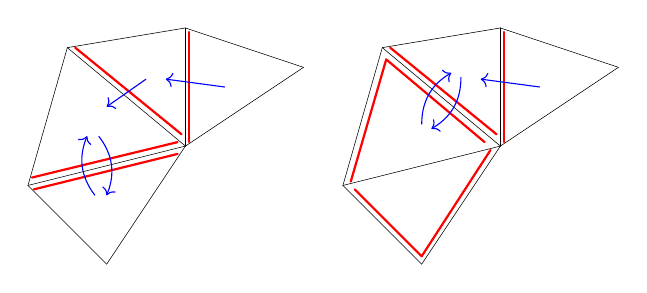
\begin{tikzpicture}[scale=0.5]
    \tkzDefPoint(2,2.5){A}
    \tkzDefPoint(5,0){B}
    \tkzDefPoint(5,3){C}
    \tkzDrawSegments(A,B B,C A,C)
    \tkzDefPoint(8,2){D}
    \tkzDrawSegments(B,D C,D)
    \tkzDefPoint(1,-1){E}
    \tkzDrawSegments(A,E B,E)
    \tkzDefPoint(3,-3){F}
    \tkzDrawSegments(E,F B,F)

    \tkzDefPoint(5.1,2.9){X}
    \tkzDefPoint(5.1,0.1){Y}
    \tkzDrawSegment[thick, color=red](X, Y)
    \tkzDefPoint(2.2, 2.5){X'}
    \tkzDefPoint(4.9, 0.3){Y'}
    \tkzDrawSegment[thick, color=red](X', Y')
    \tkzDefPoint(1.1,-0.8){M}
    \tkzDefPoint(4.8,0.1){N}
    \tkzDrawSegment[thick, color=red](M, N)
    \tkzDefPoint(1.15,-1.1){M'}
    \tkzDefPoint(4.8,-0.2){N'}
    \tkzDrawSegment[thick, color=red](M', N')

    \node (b) at (2.6, 0.5){};
    \node (a) at (2.9, -1.5){}
       edge [<-, blue, bend right=30] (b)
       ;
    \node (b) at (2.6, 0.5){}
       edge [<-, blue, bend right=30] (a)
       ;

    \draw [blue,  ->   ] (6,1.5) -- (4.5,1.7);
    \draw [blue,  ->   ] (4,1.7) -- (3,1);
    %\draw [->, blue] (2.6, 0.5) to [out=50,in=2] (2.9, -1.5);
    %\draw [->, blue] (2.8, -1.5) to [in=2,out=20] (2.5, 0.5);


    \tkzDefPoint(10,2.5){A}
    \tkzDefPoint(13,0){B}
    \tkzDefPoint(13,3){C}
    \tkzDrawSegments(A,B B,C A,C)
    \tkzDefPoint(16,2){D}
    \tkzDrawSegments(B,D C,D)
    \tkzDefPoint(9,-1){E}
    \tkzDrawSegments(A,E B,E)
    \tkzDefPoint(11,-3){F}
    \tkzDrawSegments(E,F B,F)

    \tkzDefPoint(13.1,2.9){X}
    \tkzDefPoint(13.1,0.1){Y}
    \tkzDrawSegment[thick, color=red](X, Y)
    \tkzDefPoint(10.2, 2.5){X'}
    \tkzDefPoint(12.9, 0.3){Y'}
    \tkzDrawSegment[thick, color=red](X', Y')

    \tkzDefPoint(10.1,2.2){M}
    \tkzDefPoint(12.6,0.1){N}
    \tkzDrawSegment[thick, color=red](M, N)
    \tkzDefPoint(9.2,-0.9){M'}
    \tkzDefPoint(10.1,2.2){N'}
    \tkzDrawSegment[thick, color=red](M', N')

    \tkzDefPoint(9.3,-1.1){K}
    \tkzDefPoint(11,-2.8){L}
    \tkzDrawSegment[thick, color=red](K, L)
    \tkzDefPoint(12.75,-0.1){K'}
    \tkzDefPoint(11,-2.8){L'}
    \tkzDrawSegment[thick, color=red](K', L')

    \draw [blue,  ->   ] (14,1.5) -- (12.5,1.7);
    \node (b) at (12,2){};
    \node (a) at (11,0.3){}
       edge [<-, blue, bend right=30] (b)
       ;
    \node (b) at (12,2){}
       edge [<-, blue, bend right=30] (a)
       ;
    \end{tikzpicture}
    \caption{Compatible divisibility in Dependency Graph}
    \label{Fig11}
    \end{figure}
    In \ref{Fig11}, we see a compatibility chain in a triangulation. When performing the newest vertex bisection on the right most triangle, we need to bisect its left neighboring triangle first. We obtain a recursion here since we need to bisect the triangle which our current target triangle depends on. If we successfully reached the base case, either on boundary or a cycle of size 2, we can then bisect back in an order like stack. In the example displayed in \ref{Fig11}, a base case is reached by bisecting the left most two triangles. However, a base case is not always promised. In other word, it is not guaranteed that we can always achieve either bisection on the boundary or a cycle of size 2. One example is displayed in \ref{Fig12}, and this failed in applying the newest vertex bisection, because smaller triangles are dependent on each other. That is, its dependency graph is a cycle instead of a forest, i.e. collection of trees.

    \begin{figure}[h!]
    \centering
    %\newdimen\R
    %\R=0.8cm
    \usetikzlibrary{calc}
\tikzset{
parallel segment/.style={
   segment distance/.store in=\segDistance,
   segment pos/.store in=\segPos,
   segment length/.store in=\segLength,
   to path={
   ($(\tikztostart)!\segPos!(\tikztotarget)!\segLength/2!(\tikztostart)!\segDistance!90:(\tikztotarget)$) -- 
   ($(\tikztostart)!\segPos!(\tikztotarget)!\segLength/2!(\tikztotarget)!\segDistance!-90:(\tikztostart)$)  \tikztonodes
   }, 
   % Default values
   segment pos=.5,
   segment length=18ex,
   segment distance=1mm,
},
}
    \begin{tikzpicture}[scale=0.8]
    %\draw (0:\R) \foreach \x in {60,120,...,359} {
    %            -- (\x:\R)
     %}-- cycle (90:\R) node[above] {$n=6$} ;

    \coordinate (A) at (0,0);
    \coordinate (B) at (3,0);
    \tkzDefEquilateral(B,A)\tkzGetPoint{C};
    \tkzDrawPolygon(A,B,C);
    \tkzDefEquilateral(C,A)\tkzGetPoint{D};
    \tkzDrawPolygon(A,C,D);
    \tkzDefEquilateral(C,D)\tkzGetPoint{E};
    \tkzDrawPolygon(E,C,D);
    \tkzDefEquilateral(C,E)\tkzGetPoint{F};
    \tkzDrawPolygon(C,E,F);
    \tkzDefEquilateral(C,F)\tkzGetPoint{G};
    \tkzDrawPolygon(C,F,G);
    \tkzDefEquilateral(C,G)\tkzGetPoint{H};
    \tkzDrawPolygon(C,G,H);

    %refinement edge
    \draw[red] (A) to[parallel segment] (C);
    \draw[red] (D) to[parallel segment] (C);
    \draw[red] (E) to[parallel segment] (C);
    \draw[red] (F) to[parallel segment] (C);
    \draw[red] (G) to[parallel segment] (C);
    \draw[red] (B) to[parallel segment] (C);

    %\tkzDefLine[orthogonal=through L](B,C) \tkzGetPoint{bc}
    %\tkzDefLine[orthogonal=through L](A,C) \tkzGetPoint{ac}
    %\tkzDefLine[orthogonal=through L](D,C) \tkzGetPoint{dc}
    %\tkzDefLine[orthogonal=through L](E,C) \tkzGetPoint{ec}
    %\tkzDefLine[orthogonal=through L](F,C) \tkzGetPoint{fc}
    %\tkzDefLine[orthogonal=through L](G,C) \tkzGetPoint{gc}

    %midpt
    \draw (A) -- (C) node[pos=0.5, sloped] (ac){};
    \draw (B) -- (C) node[pos=0.5, sloped] (bc){};
    \draw (D) -- (C) node[pos=0.5, sloped] (dc){};
    \draw (E) -- (C) node[pos=0.5, sloped] (ec){};
    \draw (F) -- (C) node[pos=0.5, sloped] (fc){};
    \draw (G) -- (C) node[pos=0.5, sloped] (gc){};

    %lines passing midpt
    %\draw (bc) -- (180:1);
    \draw[->,shorten >=-0.5cm, shorten <=-0.5cm, blue] (bc.south)--(bc.north);
    \draw[->,shorten >=-0.5cm, shorten <=-0.5cm, blue] (ac.north)--(ac.south);
    \draw[->,shorten >=-0.5cm, shorten <=-0.5cm, blue] (dc.north)--(dc.south);
    \draw[->,shorten >=-0.5cm, shorten <=-0.5cm, blue] (ec.north)--(ec.south);
    \draw[->,shorten >=-0.5cm, shorten <=-0.5cm, blue] (fc.south)--(fc.north);
    \draw[->,shorten >=-0.5cm, shorten <=-0.5cm, blue] (gc.south)--(gc.north);
    %\draw[thick] (C)--(B) node[pos=0.5] (x){};
    %\draw[->, blue,thick,transform canvas={rotate around={90:(x)}}] (C) -- (B) ;
    \end{tikzpicture}
    \caption{Failure of applying newest vertex bisection}
    \label{Fig12}
    \end{figure}


    \begin{lemma*}
    If the newest vertex bisection is only performed on 
    \begin{itemize}
        \item[a. ] triangles isolated in the dependency graph
        \item[b. ] pairs of mates
      \end{itemize}
    then the refinement is stable and the triangulations will be consistent.
    \end{lemma*}
    \begin{proof}
    We already proved stability in general in two dimension, and this applies here as well under a more strict condition. The consistency is obvious in compatibility divisible triangles. More specifically, if all triangles $T$ of the initial simplicial complex $\mathcal T$ are compatibly divisible, then the number of recursion is bounded. That is, we never have a cyclic dependency graph like Figure\ref{Fig12}. A detailed proof can be found in \cite{mitchell1988unified, mitchell1991adaptive}.
    \end{proof}

    \paragraph{Initial Refinement Edge}\mbox{}\\
    As described in newest vertex bisection algorithm, the start point is to pick the first peak which decides the first refinement edge. However, a determining question in this process is how we choose the first peak and initial refinement edge to produce stable and consistent triangulation after each recursion. More specifically, since we know the newest vertex bisection preserves stability generally and consistency if its dependency graph is a forest instead of cycles, the question is how to determine the initial refinement edge to promise a forest-like dependency graph. 

    One possibility is the following.
    We number the edges in any arbitrary manner. For each triangle, we always pick the edge with highest number as refinement edge. Then the dependency graph will be a forest, because with this choice of refinement edge, there can not be a cycle of length greater than two in this dependency graph.
    One approach to have a such choice is to number the edges from shortest to longest.
    Then the longest edge of each triangle in the initial simplicial complex $\mathcal T$ as the refinement edge. A consistency is proved using this approach in Kossaczky's paper \cite{kossaczky1994recursive}. Basically, he proved that the dependency graph of $\mathcal T$ is acyclic with longest edge of triangles $T\in\mathcal T$ as refinement edge.

    We may also ask whether it is even possible to choose initial refinement edges such that all triangles in the initial triangulation are compatibly divisible. In this case, the compatibility chain in the initial triangulation will have length zero (More disconnected the dependency graph is, the better strategy is).
    Finding such initial choice of refinement edges is possible. The problem can be reduced to finding a perfect matching in a graph. A detailed work and proofs can be found in \cite{mitchell1988unified,mitchell1991adaptive,mitchell201630}.
    


  \newpage
  \bibliographystyle{abbrvnat}
  \bibliography{Bib}
    
  %\subsection{}
\end{document}